\documentclass[11pt]{article}

\usepackage[margin=1in]{geometry}
\usepackage{booktabs}
\usepackage{array}
\usepackage{amsmath}
\usepackage{amssymb}
\usepackage{graphicx}
\usepackage{hyperref}
\usepackage{enumitem}
\usepackage{setspace}

\setstretch{1.03}
\setlist{nosep,leftmargin=*}
% Auto-generated by analysis.py
\newcommand{\AnalysisN}{2,912}
\newcommand{\AnalysisCounties}{707}
\newcommand{\AnalysisYears}{2019--2023}
\newcommand{\DMLIqrEffect}{0.38}
\newcommand{\PopGrowthIQR}{1.11}
\newcommand{\DescStatsRows}{%
Annual rent growth (pct. points) & 6.50 & 3.86 & 3.78 & 5.65 & 8.99 \\
Net migration rate (pct. points) & 0.51 & 1.29 & -0.16 & 0.26 & 0.95 \\
Mean annual ZORI rent (dollars) & 1443.01 & 520.95 & 1111.99 & 1351.73 & 1658.00 \\
Census population estimate & 438733.34 & 675321.08 & 142142.50 & 232477.50 & 483185.25 \\
Median household income & 84629.47 & 20978.19 & 69473.00 & 80266.00 & 96227.00 \\
Vacancy rate & 0.09 & 0.05 & 0.05 & 0.08 & 0.11 \\
Renter share & 0.33 & 0.10 & 0.25 & 0.32 & 0.38 \\
}
\newcommand{\MainResultsRows}{%
Net migration rate & 0.71 & 0.75 & 0.35 & 1.09 \\
95\% CI & [0.36, 1.06] & [0.39, 1.12] & [-0.13, 0.82] & [0.72, 1.46] \\
Observations & 2,912 & 2,912 & 2,912 & 2,794 \\
Counties & 707 & 707 & 707 & 698 \\
}
\newcommand{\HeterogeneityRows}{%
Net migration rate & 0.72 & [0.36, 1.08] \\
Net migration rate $\times$ supply constraint & 0.41 & [0.00, 0.83] \\
Observations & 2,912 &  \\
}
\newcommand{\OutcomeRMSE}{0.0236}
\newcommand{\TreatmentRtwo}{0.936}


\title{\vspace{-1.2cm}Migration Shocks and Rent Growth in Supply-Constrained Housing Markets}
\author{STAT 274 Final Project Empirical Draft}
\date{May 2026}

\begin{document}
\maketitle
\vspace{-0.7cm}

\begin{abstract}
\noindent This project studies whether pandemic-era migration shocks were associated with faster local rent growth, and whether the relationship was stronger in housing markets with tighter supply. I build a county-year panel for \AnalysisCounties{} U.S. counties over \AnalysisYears{}, combining Zillow's county-level Zillow Observed Rent Index (ZORI), Census county population estimates, and county ACS controls from Census Reporter. The treatment is net migration as a share of lagged population, and the outcome is annual log rent growth. In a two-way fixed effects model, a one percentage point increase in the net migration rate is associated with a 0.71 percentage point increase in annual rent growth; adding time-varying controls gives 0.75 percentage points. A random-forest double machine learning estimate is smaller, 0.35 percentage points, with a confidence interval that includes zero. The evidence is consistent with migration demand pressure mattering for rents, especially in constrained markets, but the results should be interpreted as observational estimates rather than a fully exogenous migration design.
\end{abstract}

\section{Motivation and Causal Question}

The COVID-19 pandemic weakened the link between workplace location and residential location for many households. At the same time, rents rose sharply in many Sun Belt, high-amenity, and lower-density markets. This project asks whether places receiving larger migration inflows experienced faster rent growth, and whether this relationship was larger in markets where housing supply was more constrained.

The main causal question is:
\[
\textit{What is the effect of pandemic-era net migration inflows on annual local rent growth?}
\]
The heterogeneity question is:
\[
\textit{Are rent effects larger in supply-constrained counties?}
\]
I treat net migration as the treatment of interest. Remote work is an important background mechanism, but this draft does not directly estimate the effect of remote-work adoption. Instead, it asks whether realized county-level population inflows translated into rent pressure. This framing is more empirically tractable because migration is measured at the county-year level and can be linked directly to local rent outcomes.

\section{Data and Variable Construction}

The empirical panel uses publicly available data sources. The outcome comes from Zillow's public research data page, which provides the ZORI county time series as a downloadable CSV and describes ZORI as a repeat-rent index for listed rental units.\footnote{\url{https://www.zillow.com/research/data/}; county ZORI CSV used by the script: \url{https://files.zillowstatic.com/research/public_csvs/zori/County_zori_uc_sfrcondomfr_sm_sa_month.csv}.} I aggregate monthly ZORI to county-year averages, requiring at least six non-missing monthly observations in a year. The outcome is annual log rent growth,
\[
Y_{ct}=\Delta \log(\text{ZORI}_{ct}).
\]

The treatment is the Census Population Estimates Program's annual net migration count divided by lagged county population.\footnote{Census county population estimates: \url{https://www2.census.gov/programs-surveys/popest/datasets/2010-2019/counties/totals/co-est2019-alldata.csv} and \url{https://www2.census.gov/programs-surveys/popest/datasets/2020-2023/counties/totals/co-est2023-alldata.csv}.} This is closer to the proposal's migration-shock concept than using total population growth because it subtracts natural increase from births and deaths:
\[
D_{ct}=\frac{\text{Net migration}_{ct}}{\text{Population}_{c,t-1}}.
\]

County characteristics come from Census Reporter's public ACS interface.\footnote{\url{https://api.censusreporter.org/1.0/data/show/latest}.} These include median household income, median gross rent, housing units, vacancy rates, renter share, and unemployment. Since these ACS controls are a latest cross-section rather than a full annual ACS panel, they are used as baseline controls in DML and to construct a supply-constraint index, not as standalone time-varying regressors in county fixed effects. The supply-constraint index averages standardized high median gross rent, high renter share, and low vacancy rate.

Appendix Table \ref{tab:desc} summarizes the final sample. Zillow county coverage is not universal; after merging sources and dropping missing values, the sample contains \AnalysisN{} county-year observations from \AnalysisCounties{} counties. Appendix Figures \ref{fig:trend} and \ref{fig:scatter} show the two main descriptive patterns: average rent growth rose sharply in 2021--2022, and county-years with higher net migration rates tend to have higher average rent growth.

\section{Identification and Estimation}

The main challenge is endogenous migration. Counties with improving labor markets, changing amenities, or local policy shocks may attract migrants and experience rent growth for reasons unrelated to migration itself. The baseline specification uses county and year fixed effects:
\[
\Delta \log(\text{Rent}_{ct}) =
\beta D_{ct} + X_{ct}'\gamma + \alpha_c + \delta_t + \varepsilon_{ct}.
\]
County fixed effects remove time-invariant local differences, while year fixed effects absorb national shocks such as inflation, mortgage-rate changes, and broad pandemic housing demand. The controlled fixed effects model includes county population, annual population growth, and lagged ZORI rent. The identifying assumption is a conditional parallel-trends-style claim: after fixed effects and controls, counties with larger net migration shocks would otherwise have had similar rent growth to counties with smaller shocks.

For heterogeneity, I estimate
\[
\Delta \log(\text{Rent}_{ct}) =
\beta D_{ct}+\theta D_{ct}S_c+X_{ct}'\gamma+\alpha_c+\delta_t+\varepsilon_{ct},
\]
where $S_c$ is the standardized supply-constraint index. A positive $\theta$ means migration inflows are associated with larger rent increases in more constrained counties.

To relax functional-form assumptions, I also estimate a partially linear double machine learning model:
\[
Y_{ct}=\theta D_{ct}+g(W_{ct})+u_{ct}, \qquad
D_{ct}=m(W_{ct})+v_{ct}.
\]
The nuisance covariates $W_{ct}$ include year indicators, population, population growth, lagged rent, ACS income, ACS median gross rent, unemployment, vacancy, renter share, and the supply-constraint index. The main nuisance learner is a random forest with five-fold cross-fitting. I also compute lasso and gradient boosting estimates as sensitivity checks. Inference uses county-clustered standard errors.

\section{Results}

Appendix Table \ref{tab:main} reports the main estimates. Coefficients are scaled as percentage-point changes in annual rent growth from a one percentage point increase in the net migration rate. The fixed effects estimates are positive and statistically distinguishable from zero. The simplest two-way fixed effects estimate is 0.71, and the controlled fixed effects estimate is 0.75. Interpreted literally, a county with a one percentage point higher net migration rate has roughly 0.7--0.8 percentage points faster annual rent growth.

The random-forest DML estimate is smaller: 0.35 percentage points, with a 95 percent confidence interval from -0.13 to 0.82. The trimmed-overlap DML estimate is larger at 1.09 percentage points. This difference suggests that the average effect is sensitive to how much weight the estimator places on counties with extreme residualized migration shocks. The interquartile range of the net migration rate is \PopGrowthIQR{} percentage points, so the main DML estimate implies that moving from the 25th to the 75th percentile of migration pressure is associated with about \DMLIqrEffect{} percentage points higher annual rent growth.

Appendix Figure \ref{fig:coef} visualizes the main estimates and two additional DML sensitivity checks. The fixed effects estimates are tightly positive. The random-forest DML and lasso DML estimates remain positive but smaller, while the boosting DML estimate is close to zero and imprecise. The sign is generally stable, but the machine-learning adjusted magnitude is model-dependent.

Appendix Table \ref{tab:het} examines heterogeneity by supply constraints. The interaction is positive: the rent response to migration is larger in counties with higher baseline rents, higher renter shares, and lower vacancy rates. Appendix Figure \ref{fig:hetero} shows the same idea descriptively. In the top migration quartile, more constrained counties have visibly higher average rent growth than less constrained counties. The interaction confidence interval is close to zero at the lower end, so this evidence is suggestive rather than decisive.

\section{Diagnostics, Limitations, and Conclusion}

The DML nuisance models predict the outcome with a cross-fitted RMSE of \OutcomeRMSE{} log points. The treatment model has an out-of-fold $R^2$ of \TreatmentRtwo{}, meaning that observed county characteristics and year indicators explain a large share of net migration variation. This is useful for adjustment, but it also warns that overlap may be limited: counties with very high inflows are systematically different from low-inflow counties.

The most important limitation is identification. Net migration is measured directly, but it is not randomly assigned. Local economic shocks, changing amenities, or expected rent appreciation could affect both migration and rent growth. Zillow also provides strong high-frequency market rent data only for counties with enough rental listings, so the sample is more urban and rental-market oriented than the full universe of U.S. counties. ACS controls are currently used as a cross-sectional county snapshot rather than as a full annual panel.

Overall, the evidence supports the core hypothesis of the proposal: migration-driven demand pressure appears to matter for local rents, especially where supply is tight. The fixed effects estimates imply that a one percentage point increase in the net migration rate corresponds to about 0.7--0.8 percentage points faster annual rent growth. A random-forest DML estimate is smaller and less precise, but still positive. The strongest next improvement would be to add sharper quasi-experimental variation, such as pre-pandemic remote-work exposure interacted with pandemic timing, and to build a full annual ACS or IRS migration panel for robustness.

\clearpage
\appendix
\setcounter{table}{0}
\setcounter{figure}{0}
\renewcommand{\thetable}{A\arabic{table}}
\renewcommand{\thefigure}{A\arabic{figure}}

\section{Tables and Figures}

\begin{table}[h!]
\centering
\small
\begin{tabular}{lccccc}
\toprule
Variable & Mean & SD & P25 & Median & P75 \\
\midrule
\DescStatsRows
\bottomrule
\end{tabular}
\caption{Descriptive statistics for the estimation panel.}
\label{tab:desc}
\end{table}

\begin{figure}[h!]
\centering
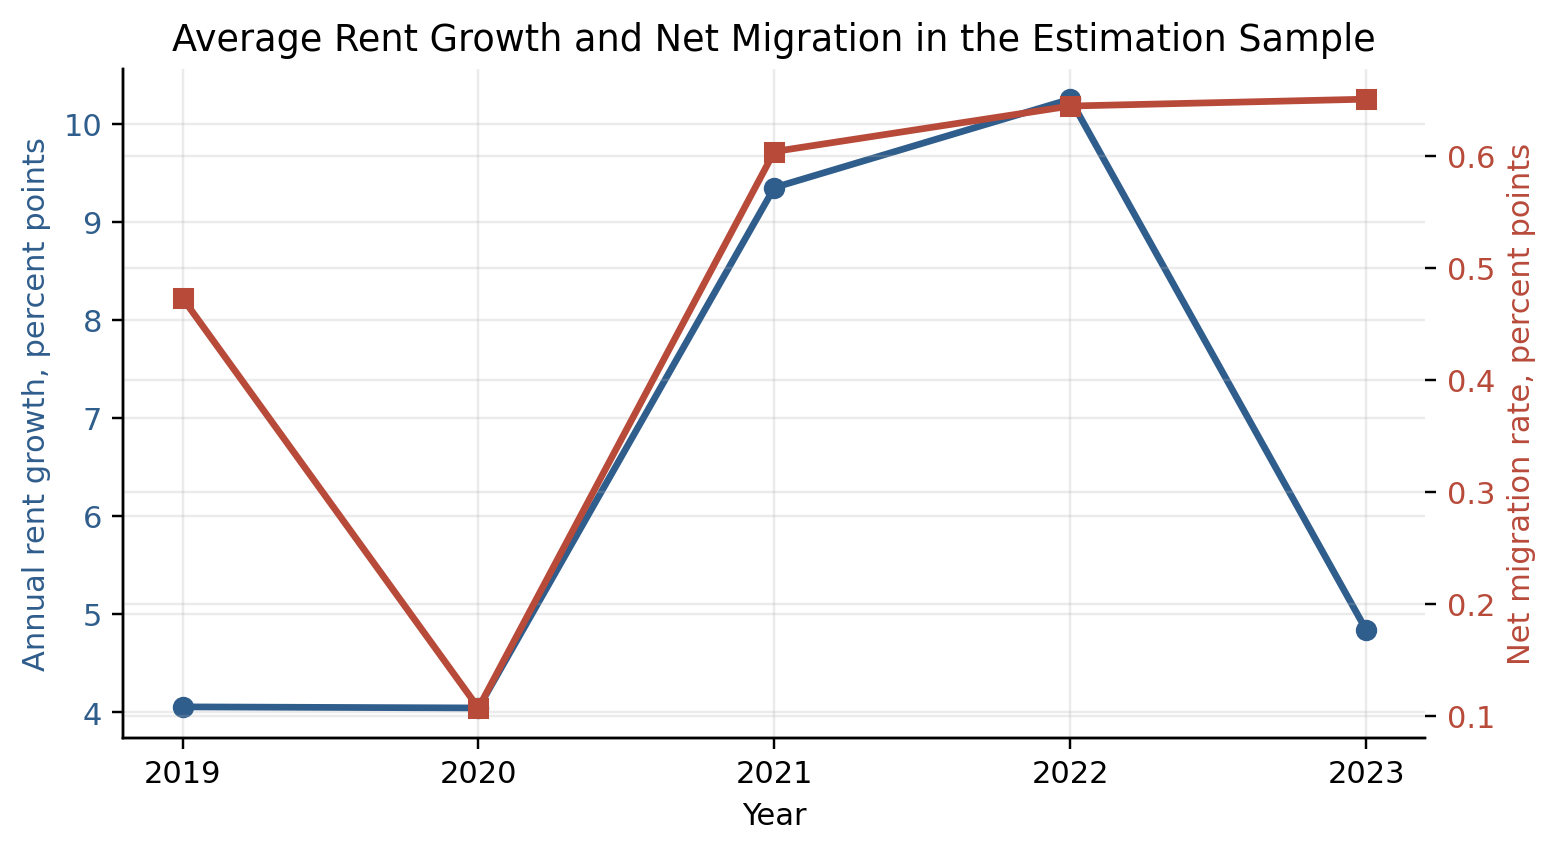
\includegraphics[width=0.86\linewidth]{results/figures/trend_rent_migration.png}
\caption{Average annual rent growth and net migration rate in the estimation sample.}
\label{fig:trend}
\end{figure}

\begin{figure}[h!]
\centering
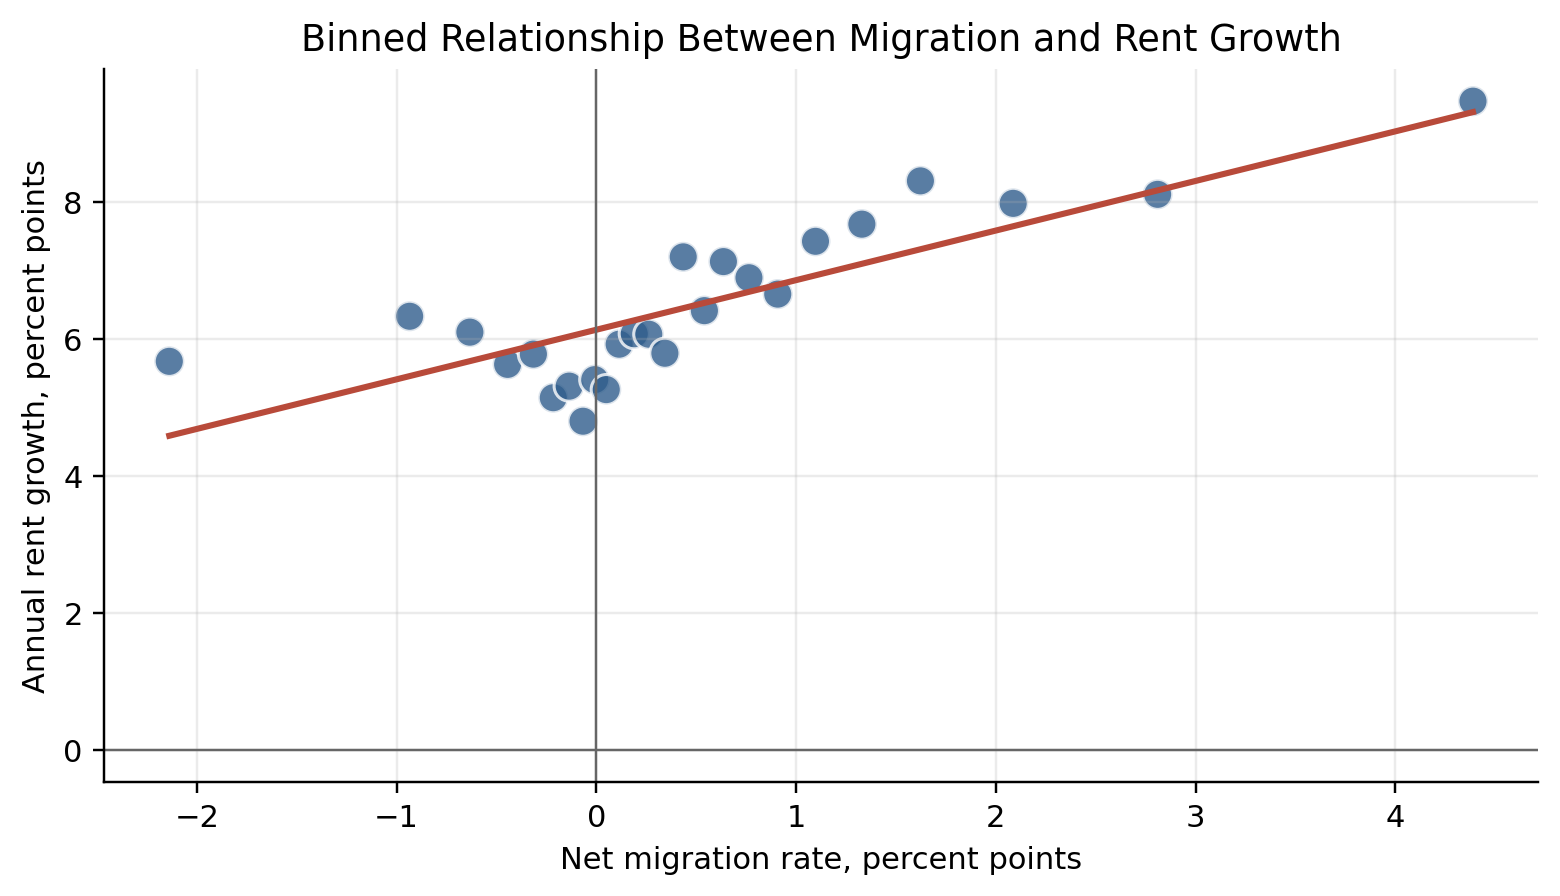
\includegraphics[width=0.86\linewidth]{results/figures/binned_scatter_migration_rent.png}
\caption{Binned relationship between net migration and annual rent growth.}
\label{fig:scatter}
\end{figure}

\begin{table}[h!]
\centering
\small
\begin{tabular}{lcccc}
\toprule
 & FE & FE + Controls & DML RF & DML RF Trimmed \\
\midrule
\MainResultsRows
County FE & Yes & Yes & No & No \\
Year FE & Yes & Yes & Yes & Yes \\
Controls & No & Time-varying & Flexible & Flexible \\
\bottomrule
\end{tabular}
\caption{Estimated effect of net migration on annual log rent growth.}
\label{tab:main}
\end{table}

\begin{figure}[h!]
\centering
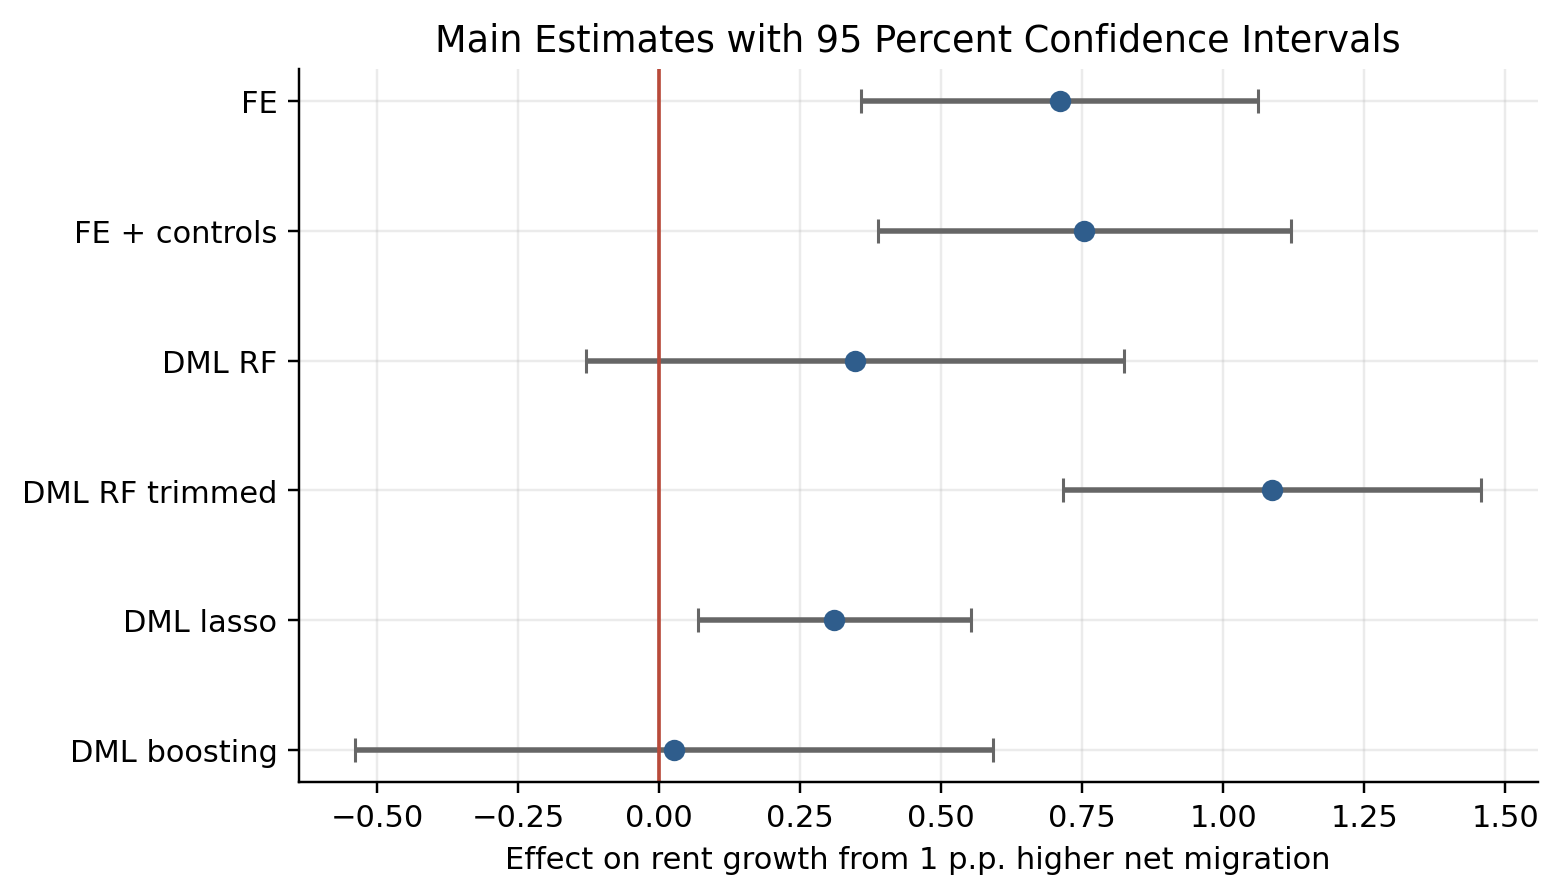
\includegraphics[width=0.86\linewidth]{results/figures/coefficient_plot.png}
\caption{Main effect estimates with 95 percent confidence intervals.}
\label{fig:coef}
\end{figure}

\begin{table}[h!]
\centering
\small
\begin{tabular}{lcc}
\toprule
 & Estimate & 95\% CI \\
\midrule
\HeterogeneityRows
County FE & Yes &  \\
Year FE & Yes &  \\
\bottomrule
\end{tabular}
\caption{Heterogeneity by the supply-constraint index.}
\label{tab:het}
\end{table}

\begin{figure}[h!]
\centering
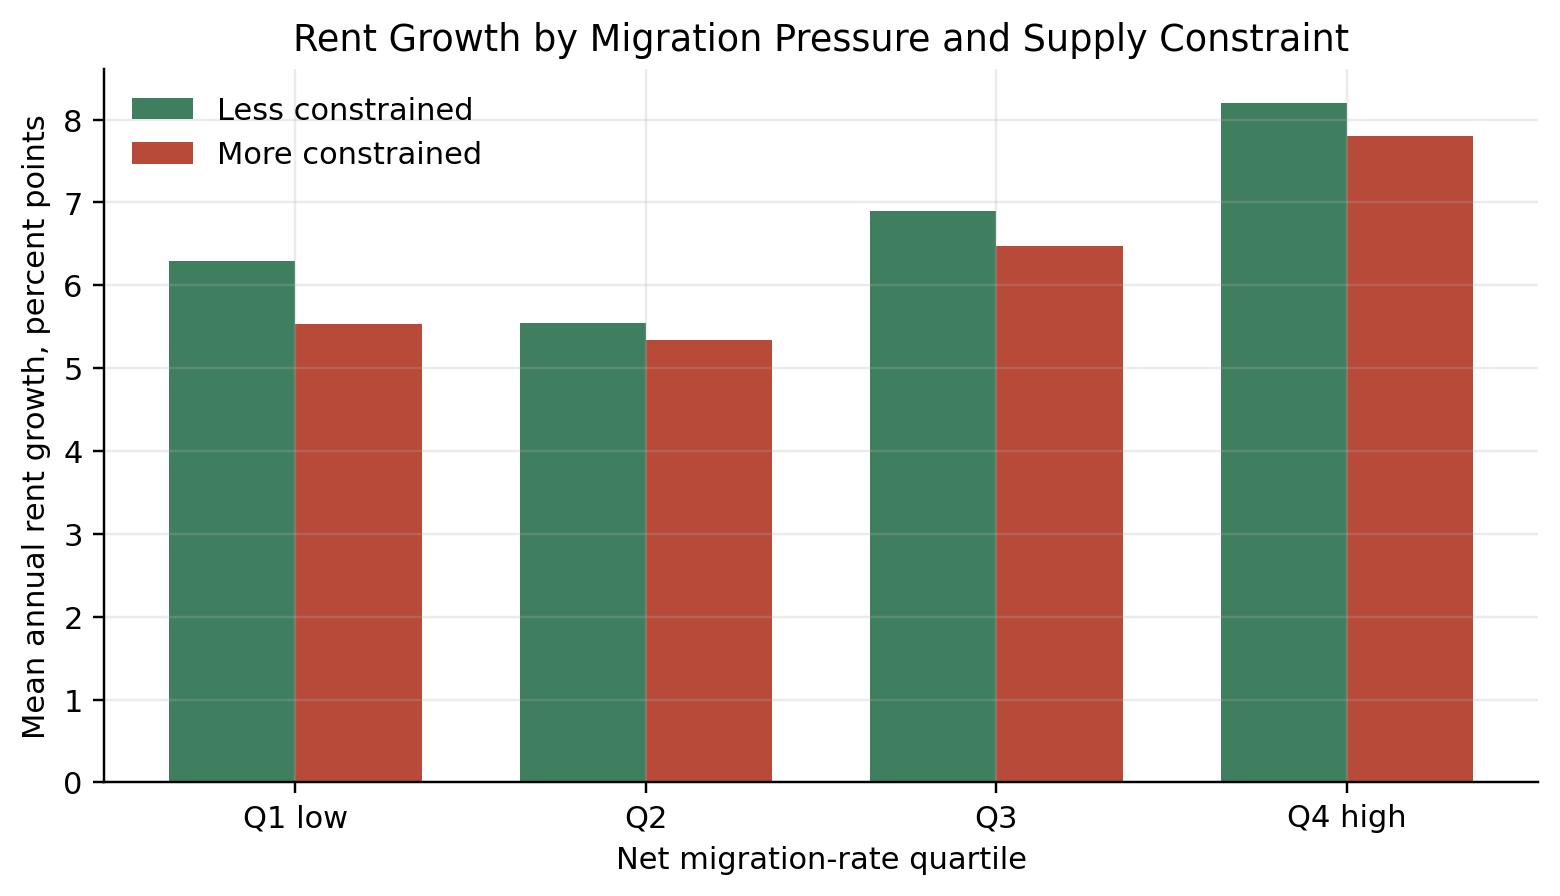
\includegraphics[width=0.86\linewidth]{results/figures/heterogeneity_quartiles.png}
\caption{Mean rent growth by migration-pressure quartile and supply-constraint group.}
\label{fig:hetero}
\end{figure}

\clearpage
\section{Reproducibility Notes}

The file \texttt{analysis.py} downloads all public inputs, constructs the analysis panel, estimates the fixed effects and DML models, generates the figures, and writes the generated LaTeX numbers used by the report. The tables can be refreshed by rerunning:
\[
\texttt{.venv/bin/python analysis.py}
\]

\section{Data Sources}

\begin{table}[h!]
\centering
\small
\begin{tabular}{p{0.26\linewidth}p{0.28\linewidth}p{0.34\linewidth}}
\toprule
Dataset & Variables Used & Role \\
\midrule
Zillow ZORI county CSV & Monthly county rent index & Primary outcome after annual aggregation \\
Census county population estimates & Population and net migration & Treatment and population controls \\
Census Reporter ACS API & Income, gross rent, housing units, vacancy, renter share, unemployment & DML controls and supply-constraint index \\
\bottomrule
\end{tabular}
\caption{Public data sources used in this empirical draft.}
\end{table}

\end{document}
